%!TEX root = ../OGUSAdoc.tex

Among households in \ogindia, we model both age heterogeneity and within-age ability heterogeneity. We use this ability or productivity heterogeneity to generate the income heterogeneity that we see in the data.

Differences among workers' productivity in terms of ability is one of the key dimensions of heterogeneity to model in a micro-founded macroeconomy. In this chapter, we characterize this heterogeneity as deterministic lifetime productivity paths to which new cohorts of agents in the model are randomly assigned. In \ogindia, households' labor income comes from the equilibrium wage and the agent's endogenous quantity of labor supply. In this section, we augment the labor income expression with an individual productivity $e_{j,s}$, where $j$ is the index of the ability type or path of the individual and $s$ is the age of the individual with that ability path.
\begin{equation}\tag{\ref{EqTaxCalcLabInc}}
  \text{labor income:}\quad x_{j,s,t}\equiv w_t e_{j,s}n_{j,s,t} \quad\forall j,t \quad\text{and}\quad E+1\leq s\leq E+S
\end{equation}
In this specification, $w_t$ is an equilibrium wage representing a portion of labor income that is common to all workers. Individual quantity of labor supply is $n_{j,s,t}$, and $e_{j,s}$ represents a labor productivity factor that augments or diminishes the productivity of a worker's labor supply relative to average productivity.

We calibrate deterministic ability paths such that each lifetime income group has a different life-cycle profile of earnings. The distribution on income and wealth are often focal components of macroeconomic models. As such, we use a calibration of deterministic lifetime ability paths from \citet{DeBackerEtAl:2017b} that can represent U.S. earners in the top 1\% of the distribution of lifetime income. \citet{PikettySaez:2003} show that income and wealth attributable to these households has shown the greatest growth in recent decades. The data come from the U.S. Internal Revenue Services's (IRS) Statistics of Income program (SOI) Continuous Work History Sample (CWHS). \citet{DeBackerEtAl:2017b} match the SOI data with Social Security Administration (SSA) data on age and Current Population Survey (CPS) data on hours in order to generate a non-top-coded measure of hourly wage.

\begin{figure}[htbp]\centering \captionsetup{width=4.0in}
  \caption{\label{FigLogAbil}\textbf{Exogenous life cycle income ability paths $\log(e_{j,s})$ with $S=80$ and $J=7$}}
  \fbox{\resizebox{4.0in}{3.0in}{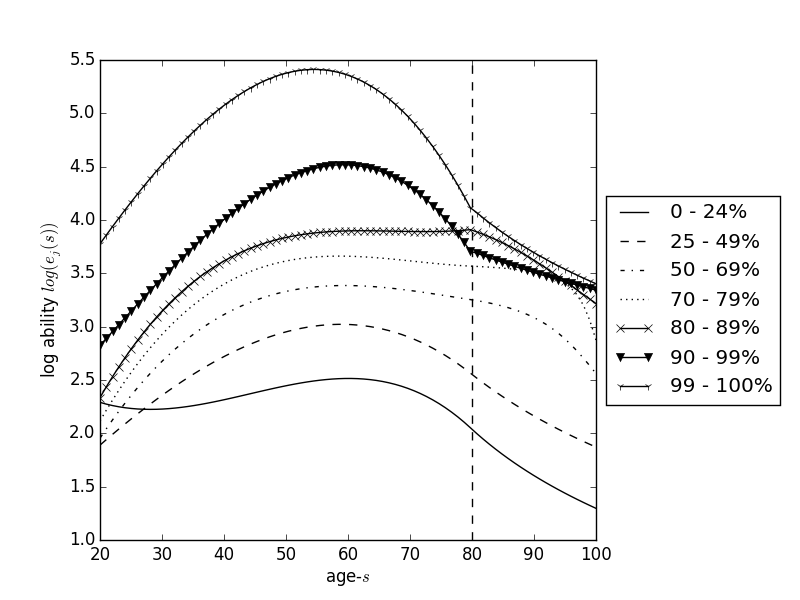
\includegraphics{images/ability_log_2D.png}}}
\end{figure}

Figure \ref{FigLogAbil} shows a calibration for $J=7$ deterministic lifetime ability paths $e_{j,s}$ corresponding to labor income percentiles $\bm{\lambda}=[0.25, 0.25, 0.20, 0.10, 0.10, 0.09, 0.01]$. Because there are few individuals above age 80 in the data, \citet{DeBackerEtAl:2017b} extrapolate these estimates for model ages 80-100 using an arctan function.

We calibrate the model such that each lifetime income group has a different life-cycle profile of earnings. Since the distribution on income and wealth are key aspects of our model, we calibrate these processes so that we can represent earners in the top 1 percent of the distribution of lifetime income. It is income and wealth attributable to these households that has shown the greatest growth in recent decades (see, for example, \citet{PikettySaez:2003}). In order to have observations on the earnings of those at very top of the distribution that are not subject to top-coding we use data from the Internal Revenue Services's (IRS) Statistics of Income program (SOI).


\section{Continuous Work History Sample}\label{SecLFEarnCWHS}

  The SOI data we draw from are the Continuous Work History Sample (CWHS).  From this CWHS, we use a panel that is a 1-in-5000 random sample of tax filers from 1991 to 2009.  For each filer-year observation we are able to observe detailed information reported on Form 1040 and the associated forms and schedules.  We are also able to merge these tax data with Social Security Administration (SSA) records to get information on the age and gender of the primary and secondary filers.  Our model variable of effective labor units maps into wage rates, because the market wage rate in the model, $w_{t}$, is constant across households.  Earnings per hour thus depend upon effective labor units and equal $e_{j,s,t}\times w_{t}$ for household in lifetime income group $j$, with age $s$, in year $t$.  Income tax data, however, do not contain information on hourly earnings or hours works.  Rather, we only observe total earned income (wage and salaries plus self-employment income) over the tax year.  In order to find hourly earnings for tax filers, we use an imputation procedure.  This is described in detail in \citet{DeBackerRamnath:2017}.  The methodology applies an imputation for hours worked for a filing unit based on a model of hours worked for a filing unit estimated from the Current Population Survey (CPS) for the years 1992-2010.\footnote{The CPS survey asks retrospective questions about income in the last year and average hours worked per week (and weeks worked) in the last year).  Therefore, these CPS surveys line up with tax years 1991-2009.} We then use the imputed hours to calculate hourly earnings rates for tax filing units in the CWHS.

  We exclude from our sample filer-year observations with earned income (wages and salaries plus business income) of less than \$1,250. We further exclude those with positive annual wages, but with hourly wages below \$5.00 (in 2005\$). We also drop one observation where the hourly wage rate exceeds \$25,000.\footnote{This threshold is equivalent to \$50 million of wage income in one year at full time (40 hours per week) of work.} Economic life in the model runs from age 21 to 100. Our data have few observations on filers with ages exceeding 80 years old. Our sample is therefore restricted to those from ages 21 to 80. After these restrictions, our final sample size is 333,381 filer-year observations.


\section{Lifetime Income}\label{SecLFearnLifInc}

  In our model, labor supply and savings, and thus lifetime income, are endogenous. We therefore define lifetime income as the present value of lifetime labor endowments and not the value of lifetime labor earnings. Note that our data are at the tax filing unit.  We take this unit to be equivalent to a household.  Because of differences in household structure (i.e., singles versus couples), our definition of lifetime labor income will be in per adult terms.  In particular, for filing units with a primary and secondary filer, our imputed wage represents the average hourly earnings between the two. When calculating lifetime income we assign single and couple households the same labor endowment.  This has the effect of making our lifetime income metric a per adult metric, there is therefore not an over-representation of couple households in the higher lifetime income groups simply because their time endowment is higher than for singles. We use the following approach to measure the lifetime income.

  First, since our panel data do not allow us to observe the complete life cycle of earnings for each household (because of sample attrition, death or the finite sample period of the data), we use an imputation to estimate wages in the years of the household's economic life for which they do not appear in the CWHS. To do this, we estimate the following equation, separately by household type (where household types are single male, single female, couple with male head, or couple with female head):
  \begin{equation}\label{eqn:wage_step1}
    ln(w_{i,t}) = \alpha_{i} + \beta_{1}age_{i,t} + \beta_{2}age_{i,t}^{2} + \beta_{3}*age_{i,t}^{3} + \varepsilon_{i,t}
  \end{equation}

  \begin{table}[htbp]\centering\captionsetup{width=5.8in}
    \caption{\label{tab:wage_step1}\textbf{Initial Log Wage Regressions}}
    \begin{threeparttable}
    \begin{tabular}{>{\scriptsize}l |>{\scriptsize}c >{\scriptsize}c >{\scriptsize}c >{\scriptsize}c}
    \hline\hline
    \multicolumn{1}{c}{\scriptsize{Dependent}} & Single & Single & Married, & Married, \\[-2mm]
    \multicolumn{1}{c}{\scriptsize{variables}}  & males & females & male head  & female head \\
    \hline
    $Age$ & 0.177*** & 0.143*** & 0.134*** & 0.065** \\
          & (0.006) & (0.005) & (0.004) & (0.027) \\
    $Age^{2}$ & -0.003*** & -0.002*** & -0.002*** & -0.000 \\
              & (0.000) & (0.000) & (0.000) & (0.001) \\
    $Age^{3}$ & 0.000*** & 0.000*** & 0.000*** & 0.000 \\
              & (0.000) & (0.000) & (0.000) & (0.000) \\
    Constant & -0.839*** & -0.648*** & -0.042 & 1.004*** \\
             & (0.072) & (0.070) & (0.058) & (0.376) \\
    \hline
    Adj $R^{2}$  & -0.007 & 0.011 & -0.032 & -0.324 \\
    Observations & 88,833 & 96,670 & 141,564 & 6,314 \\
    \hline\hline
    \end{tabular}
    \begin{tablenotes}
      \scriptsize{\item[]Source: CWHS data, 1991 -- 2009.
      \item[**]Significant at the 5 percent level ($p<0.05$).
      \item[***]Significant at the 1 percent level ($p<0.01$).}
    \end{tablenotes}
    \end{threeparttable}
  \end{table}

  The parameter estimates, including the household fixed effects, from Equation \ref{eqn:wage_step1} are shown in Table \ref{tab:wage_step1}. These estimates are then used to impute values for log wages in years of each households' economic life for which we do not have data.  This creates a balanced panel of log wages of households with heads aged 21 to 80. The actual and imputed wage values are then used to calculate the net present value of lifetime labor endowments per adult for each household. Specifically, we define lifetime income for household $i$ as:

  \begin{equation}\label{eqn:LI}
    LI_{i} = \sum_{t=21}^{80}\left(\frac{1}{1+r}\right)^{t-21}(w_{i,t}*4000)
  \end{equation}

  \noindent\noindent Note that households are all have the same time endowment in each year (4000 hours).  Thus the amount of the time endowment scales lifetime income up or down, but does not change the lifetime income of one household relative to another. This is not the case with the interest rate, $r$, which we fix at 4\%. Changes in the interest rate differentially impact the lifetime income calculation for different individuals because they may face different earnings profiles. For example, a higher interest rate would reduced the discounted present value of lifetime income for those individuals whose wage profiles peaked later in their economic life by a larger amount than it would reduce the discounted present value of lifetime income for individuals whose wage profiles peaked earlier.


\section{Profiles by Lifetime Income}

  With observations of lifetime income for each household, we next sort households and find the percentile of the lifetime income distribution that each household falls in.  With these percentiles, we create our lifetime income groupings.
  \begin{equation}\label{EqLfEarnLambda_j}
    \lambda_{j}=[0.25, 0.25, 0.2, 0.1, 0.1, 0.09, 0.01]
  \end{equation}
  That is, lifetime income group one includes those in below the 25th percentile, group two includes those from the 25th to the median, group three includes those from the median to the 70th percentile, group four includes those from the 70th to the 80th percentile, group 5 includes those from the 80th to 90th percentile, group 6 includes those from the 90th to 99th percentile, and group 7 consists of the top one percent in the lifetime income distribution.  Table \ref{tab:li_group_stats} presents descriptive statistics for each of these groups.

  \begin{table}[htbp] \centering \captionsetup{width=6.0in}
  \caption{\label{tab:li_group_stats}\textbf{Descriptive Statistics by Lifetime Income Category}}
    \begin{threeparttable}
    \begin{tabular}{>{\scriptsize}l |>{\scriptsize}r >{\scriptsize}r >{\scriptsize}r >{\scriptsize}r >{\scriptsize}r >{\scriptsize}r >{\scriptsize}r >{\scriptsize}r}
      \hline\hline
      \multicolumn{1}{c}{\scriptsize{Lifetime Income}} & & & & & & & & \\
      \multicolumn{1}{c}{\scriptsize{Category:}} & \multicolumn{1}{c}{\scriptsize{1}} & \multicolumn{1}{c}{\scriptsize{2}} & \multicolumn{1}{c}{\scriptsize{3}} & \multicolumn{1}{c}{\scriptsize{4}} & \multicolumn{1}{c}{\scriptsize{5}} & \multicolumn{1}{c}{\scriptsize{6}} & \multicolumn{1}{c}{\scriptsize{7}} & \multicolumn{1}{c}{\scriptsize{All}} \\
      \hline
      Percentiles & 0-25  & 25-50 & 50-70 & 70-80 & 80-90 & 90-99 & 99-100 & 0-100 \\
      Observations & 65,698 & 101,484 & 74,253 & 33,528 & 31,919 & 24,370 & 2,129 & 333,381 \\
      Fraction Single & & & & & & & & \\
      \ \ \ Females & 0.30  & 0.24  & 0.25  & 0.32  & 0.38  & 0.40  & 0.22  & 0.28 \\
      \ \ \  Males & 0.18  & 0.22  & 0.30  & 0.35  & 0.38  & 0.37  & 0.20  & 0.26 \\
      Fraction Married & & & & & & & & \\
      \ \ \ Female Head & 0.08  & 0.00  & 0.00  & 0.00  & 0.00  & 0.00  & 0.00  & 0.02 \\
      \ \ \ Male Head & 0.45  & 0.53  & 0.45  & 0.32  & 0.23  & 0.23  & 0.57  & 0.39 \\
      Mean: & & & & & & & & \\
      Age, Primary & 51.72 & 44.15 & 38.05 & 34.09 & 31.53 & 30.79 & 40.17 & 39.10 \\
      Hourly Wage & 11.60 & 16.98 & 20.46 & 23.04 & 26.06 & 40.60 & 237.80 & 21.33 \\
      Annual Wages & 25,178 & 44,237 & 54,836 & 57,739 & 61,288 & 92,191 & 529,522 & 51,604 \\
      Lifetime Income & 666,559 & 1,290,522 & 1,913,029 & 2,535,533 & 3,249,287 & 5,051,753 & 18,080,868 & 2,021,298 \\
      \hline\hline
    \end{tabular}%
    \begin{tablenotes}
      \tiny{\item[*] CWHS data, 1991-2009, all nominal values in 2005\$.}
    \end{tablenotes}
    \end{threeparttable}
  \end{table}

  To get a life-cycle profile of effective labor units for each group, we estimate the wage profile for each lifetime income group.  We do this by estimating the following regression model separately for each lifetime income group using data on actual (not imputed) wages:
  \begin{equation}\label{eqn:wage_profile}
    ln(w_{i,t})=\alpha +  \beta_{1}age_{i,t} + \beta_{2}age_{i,t}^{2} + \beta_{3}*age_{i,t}^{3}+ \varepsilon_{i,t}
  \end{equation}
  The estimated parameters from equation \eqref{eqn:wage_profile} are given in Table \ref{tab:wage_profiles}. The life-cycle earnings profiles implied by these parameters are plotted in Figure \ref{FigLogAbil}. Note that there are few individuals above age 80 in the data. To extrapolate these estimates for model ages 80-100, we use an arctan function of the following form:
  \begin{equation}\label{EqLfEarnArctan}
    y = \left(\frac{-a}{\pi}\right)*arctan(bx+c)+\frac{a}{2}
  \end{equation}
  where $x$ is age, and $a$, $b$, and $c$ are the parameters we search over for the best fit of the function to the following three criteria: 1) the value of the function should match the value of the data at age 80 2) the slope of the arctan should match the slope of the data at age 80 and 3) the value of the function should match the value of the data at age 100 times a constant.  This constant is .5 for all lifetime income groups, except the 2nd highest ability is .7 (otherwise, the 2nd highest has a lower income than the 3rd highest ability group in the last few years).

  \begin{table}[htbp] \centering \captionsetup{width=6.0in}
  \caption{\label{tab:wage_profiles}\textbf{Log Wage Regressions, by Lifetime Income Group}}
    \begin{threeparttable}
    \begin{tabular}{>{\scriptsize}l |>{\scriptsize}c >{\scriptsize}c >{\scriptsize}c >{\scriptsize}c |>{\scriptsize}c}
      \hline\hline
      \multicolumn{1}{c}{\scriptsize{Lifetime}} & & & & & \\
      \multicolumn{1}{c}{\scriptsize{income groups}}   & & & & & \\
      \multicolumn{1}{c}{\scriptsize{(percentiles)}} & Constant & $Age$ & $Age^2$ & $Age^3$ & Observations \\
      \hline
      0 to 25 & 3.41000000*** & -0.09720122*** & 0.00247639*** & -0.00001842*** & 65,698 \\
              & (0.08718100) & (0.00543339) & (0.00010901) & (0.00000071) &  \\
      25 to 50 & 0.69689692*** & 0.05995294*** & -0.00004086 & -0.00000521*** & 101,484 \\
            & (0.05020758) & (0.00345549) & (0.00007627) & (0.00000054) &  \\
      50 to 70 & -0.78761958*** & 0.17654618*** & -0.00240656*** & 0.00001039*** & 74,253 \\
               & (0.04519637) & (0.00338371) & (0.00008026) & (0.00000061) &  \\
      70 to 80 & -1.11000000*** & 0.21168263*** & -0.00306555*** & 0.00001438*** & 33,528 \\
            & (0.06838352) & (0.00530190) & (0.00012927) & (0.00000099) &  \\
      80 to 90  & -0.93939272*** & 0.21638731*** & -0.00321041*** & 0.00001579*** & 31,919 \\
            & (0.08333727) & (0.00664647) & (0.00016608) & (0.00000130) &  \\
      90 to 99 & 1.60000000*** & 0.04500235*** & 0.00094253*** & -0.00001470*** & 24,370 \\
            & (0.11723131) & (0.00931334) & (0.00022879) & (0.00000176) &  \\
      99 to 100 & 1.89000000*** & 0.09229392** & 0.00012902 & -0.00001169* & 2,129 \\
            & (0.50501510) & (0.03858202) & (0.00090072) & (0.00000657) &  \\
      \hline\hline
    \end{tabular}
    \begin{tablenotes}
      \scriptsize{\item[]Source: CWHS data, 1991 -- 2009.
      \item[*]Significant at the 10 percent level ($p<0.10$).
      \item[**]Significant at the 5 percent level ($p<0.05$).
      \item[***]Significant at the 1 percent level ($p<0.01$).}
    \end{tablenotes}
    \end{threeparttable}
  \end{table}
